\documentclass[conference]{IEEEtran}
%\usepackage[latin1]{inputenc}
\usepackage{amsmath}
\usepackage{amsfonts}
\usepackage{amssymb}
\usepackage{graphicx}
\usepackage{epstopdf}
\usepackage{AMMALanguages}
\usepackage[table]{xcolor}
\usepackage{tabularx}
\usepackage{booktabs}
\usepackage{cleveref}
\usepackage{url}

\usepackage[normalem]{ulem} % for \sout
\usepackage{xcolor}
\definecolor{colgray}{gray}{0.75}

% Put edit comments in a really ugly standout display
\usepackage{ifthen}
\usepackage{amssymb}
\newboolean{showcomments}
\setboolean{showcomments}{true} % toggle to show or hide comments
\ifthenelse{\boolean{showcomments}}
  {\newcommand{\nb}[2]{
    \fcolorbox{gray}{yellow}{\bfseries\sffamily\scriptsize#1}
    {$\blacktriangleright$#2$\blacktriangleleft$}
   }
   \newcommand{\version}{\emph{\scriptsize$-$working$-$}}
  }
  {\newcommand{\nb}[2]{}
   \newcommand{\version}{}
  }

\newcommand\rs[1]{\nb{levi}{\textsl{#1}}}
\newcommand\mf[1]{\nb{manuel}{\textsl{#1}}}
\newcommand\mc[1]{\nb{bentley}{\textsl{#1}}}




\newcommand{\chunk}[2]{%
	\fcolorbox{black}{yellow}{\bfseries\sffamily\scriptsize#1}%
   {$\blacktriangleright$#2$\blacktriangleleft$}%
}

\newcommand{\bentley}[1]{\chunk{Bentley}{\textbf{\textcolor{green}{\textsl{#1}}}}}
\newcommand{\levi}[1]{\chunk{Levi}{\textbf{\textcolor{red}{\textsl{#1}}}}}
\newcommand{\cgg}[1]{\chunk{Claudio}{\textbf{\textcolor{blue}{\textsl{#1}}}}}
\newcommand{\javi}[1]{\chunk{Javi}{\textbf{\textcolor{brown}{\textsl{#1}}}}}

\begin{document}
\title{SyVOLT - A Model Transformation Verifier}
%\title{Full Verification of Model Transformation Contracts for Declarative ATL}
\author{Levi L\'{u}cio, Bentley James Oakes, Cl\'{a}udio Gomes, Hans Vangheluwe}

\author{\IEEEauthorblockN{Levi L\'{u}cio\IEEEauthorrefmark{1},
			Bentley James Oakes\IEEEauthorrefmark{1},
			Claudio Gomes\IEEEauthorrefmark{2} and
			Hans Vangheluwe$^{\dagger,*}$}
		\IEEEauthorblockA{\IEEEauthorrefmark{1}School of Computer Science,
			McGill University,
			Canada\\ levi@cs.mcgill.ca, bentley.oakes@mail.mcgill.ca}
		\IEEEauthorblockA{\IEEEauthorrefmark{2}MSDL Lab,
			University of Antwerp,
			Belgium\\ claudio.goncalvesgomes@ua.ac.be, hans.vangheluwe@ua.ac.be}	
	}

\date{\today}


\maketitle 

%\tableofcontents



\begin{abstract}
 
We introduce SyVOLT, a plugin for the Eclipse development environment for the verification of structural contracts on model transformations. The plugin allows the user to build transformations in our transformation language DSLTrans using a visual editor. The pre-/post- condition contracts to be proved on the transformation can also be built in a similar interface.

Our contract proving process is exhaustive, meaning that if a contract is said to hold, then the contract will hold for all input models of a transformation. If the contract will not hold, then the input model counter-examples where the contract fails will be presented.

Demo: \url{https://www.youtube.com/watch?v=8PrR5RhPptY}



\end{abstract}


\section{Introduction}
\label{sec:intro}
% Graph-based model transformations have become in the last few years the main
% means for manipulating models in model-driven development. Their simplicity,
% their allowance for mathematical treatment, and the fact that they can natively
% manipulate domain-specific concepts expressed in metamodels, all make
% graph-based model transformations an excellent compromise between strong
% theoretical foundations and applicability to real-world problems.
% Because of the importance of graph-based model transformations both in the
% academic and the industrial arenas, their verification is of prime importance.
Model transformations are at the center of model-driven development, making
pragmatic and usable tools for their verification indispensable. In this paper
we introduce SyVOLT (Symbolic Verifier of mOdeL Transformations)~\cite{syvolt},
an Eclipse plugin that allows verifying pre / post-condition structural
contracts on model transformations. SyVOLT's operation relies on a theoretical framework
that has been developed for the DSLTrans model transformation language. In this
framework, pre / post-condition contracts can be shown to either hold for all
input/output pairs resulting from executing a given DSLTrans model
transformation, or not to hold for at least one of those input/output
pairs~\cite{Lucio2014}.

% A fully
% automatic property prover based on this theory has been shown to be applicable
% to industrial problems~\cite{Selim2014}.

Extensive work exists on the verification of different aspects of model
transformations~\cite{AmraniLSCDVTC12}. In~\cite{Vallecillo2012} the
authors describe a method where `Tracts' can be specified for model
transformations. Tracts resemble SyVOLT's contracts and define a set
of constraints on the source and target metamodels, a set of source-target constraints, and a tract test suite, i.e., a collection of source models
satisfying the source constraints. The accompanying TractsTool can then
automatically test the transformation by verifying if all source/target model
pairs satisfy the constraints in the tract test suite.
Several other approaches support the testing of model transformations based
on different kinds of contracts such as model fragments~\cite{Mottu2008}, graph
patterns~\cite{Guerra12,BaloghBCGHMPPRVa10}, Triple Graph Grammars (TGGs)~\cite{WieberAS14} or dedicated testing
languages~\cite{Garcia-Dominguez11}. 

The tool described in \cite{Buettner2013} automatically transforms
transformations in a number of transformation languages (such as ATL) to OCL. Verification is then
done using a model finder which will attempt to find a counter-example to the
property being proved. Anastasakis et al.~\cite{Anastasakis07}
translate model transformations to Alloy in order to verify if given
assertions hold for the given transformations. Both these
approaches attempt to exhaustively verify the model transformation, as SyVOLT
does. However, while SyVOLT guarantees that all counter-examples to a contract
are always found, this is not granted by the two approaches introduced above.

The distinguishing feature of SyVOLT is that, unlike the methods described
above, our tool allows for contracts to be proved for all possible
transformation executions, i.e., for all possible input models.
However, we share with most tools described above the same implication idea: the
pre-condition of a contract sets constraints on the input models to the
transformation, and the post-condition defines constraints on the output model.







\section{Highlights}
\label{sec:highlights}
SyVOLT has a number of unique features, outlined below.

\subsection{Graphical Modelling of Model Transformation Contracts}

SyVOLT proves pre-/post-condition contracts hold for a model transformation.
Such contracts establish relations between patterns occurring in input and output
models of a model transformation. If a contract holds, then a formal guarantee
exists that whenever an input model contains the pattern specified in the
pre-condition of the contract, the output model contains the pattern specified
in the post-condition part of the contract and any traceability relations
between the two. Due to the graph-like structure of the pre and post conditions
of contracts, the visual representation of the contract in SyVolt editor allows
the user to quickly build and intuitively understand their meaning.
%If a textual (logical or mathematical) editor where to be used, the user would
%need an extra system of identifiers to correctly prescribe the associations
% between pre and post-condition elements whereas in the visual representation, the user graphically builds the associations between those elements.
%\levi{Claudio, I don't understand this sentence}
%\cgg{Please tell me now if you can understand it.}

%The visual representation of a contract has all the necessary information to
% derive the correct logical expression to be used by the internal SyVolt prover.

\subsection{Push-Button Proofs}
\label{sec:push_button_proofs}
SyVOLT is a verification tool that provides formal guarantees of correctness of
a model transformation. The proving process is fully automatic and
the all formal details are completely hidden from the user, who only needs to specify a
set of contracts for the transformation being verified. Once the transformation and the
contracts of interest are created, one command will start the property proving
process. This process will automatically create all required artifacts (as
detailed in the following section), run the process, and then provide the
results to the user within the Eclipse environment, as seen in
Figure~\ref{fig:output}. This allows the user to continually stay within the
Eclipse environment, which is where he develops the contracts and the model
transformations.

\subsection{Based on Symbolic Execution}

Our technique shares its principles with symbolic execution, a classic method to
verify code. The underlying idea entails building a finite representation of the
(infinite) set of computations that can be built by a model transformation
specification. In this context, each symbolic execution (also called
\emph{path condition}) consists of a combination of a subset of the rules of the
model transformation being verified in a way that it represents the execution of the the model transformation over any input
model those rules match on. Then, properties of interest can be proved on the
set of generated path conditions and extrapolated to the infinite set of the
model transformation's potential computations.

% Our model transformation verification technique relies on models as the
% means to internally represent both symbolic executions and contracts. SyVOLT
% then reasons over these graphs to build a proof that contracts hold or do not
% hold.

% Note that by using a typed graph representation, our technique can prove
% contracts that include constraints on the structure and the attributes of the
% input and output models. 

% \levi{keep the text from here on?} An example of this would be in the
% Families-To-Persons transformation from the ATL zoo [CITE]. In this transformation, the name for a person in the
% output graph is a concatenation of two strings \cgg{instead of ''strings``,
% should be ''attributes``} from elements in the input graph. Our contract prover
% can prove that this concatenation will be valid in all cases.

\begin{figure}
\centering
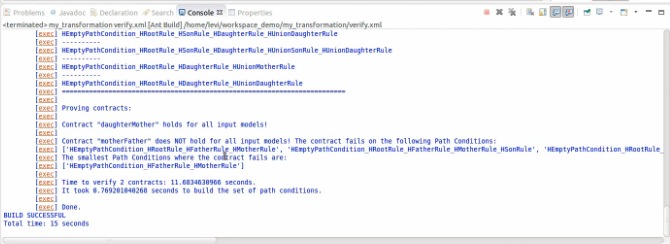
\includegraphics[width=0.5\textwidth]{figures/output}
\caption{The results of the contract prover}
\label{fig:output}
\end{figure}

\subsection{Input Independence and Exhaustiveness} 

Our technique is exhaustive, in the sense that whenever a contract holds, it
will hold for all possible input models to a transformation. This is possible
because SyVOLT operates on specifications of outplace model transformations
where unbounded loops and model element deletions are not allowed. SyVOLT thus proves
contracts in an input-independent manner, relying only on the specification of the
transformation. The soundness and completeness of our technique is described
in~\cite{Lucio2014}.

\subsection{Proving Contracts about ATL Model Transformations}
The Atlas Transformation Language (ATL)~\cite{atlTool} is commonly-used in both
industry and academia applications. In order to extend our approach into these domains, we
have developed a higher-order transformation that is able to automatically
transform declarative ATL transformations into our transformation language
DSLTrans~\cite{Oakes}. This allows the user to also prove contracts on
ATL transformations.

\subsection{Scalability and Speed}

We have some evidence that SyVOLT scales to transformations of practical
interest. This has been empirically shown by applying it to DSLTrans
transformations with up to over 60 rules, and ATL transformations with up to 13
rules~\cite{Oakes}. From our own experience with DSLTrans, the size of a
DSLTrans transformations varies widely, with the average size ranging from 10 up
to 50 rules. The average size of an ATL transformation is around 20 rules. [cite
Manuel's paper, should we keep this?] \cgg{The problem is that there is not enough infor about those 20 rules. Are they imperative? Do they use imperative helpers? How many rules are generated when those transformations are translated to DSLTrans?}.
Even though our technique is exhaustive, our approach takes relatively short
amounts of time to prove contracts. For example, our experiments with industrial
transformations~\cite{Oakes} show that contracts can be verified within a few
minutes. In Gehan Selim's PhD thesis~\cite{Selim2015}
further evidence of SyVOLT's speed is given when verifying a relatively large
model transformation for giving semantics to the UML-RT language in terms of
the Kiltera process language~\cite{PosseDingel2014}. SyVOLT's symbolic execution
engine is fully homegrown~\cite{LucioVang} and does not depend on third-party
solvers \cgg{This sentence and the next one are part of the "how". Hence, they should be in the Architecture section. The highlight here is the speed and not how that performance was achieved. Correct?}. Although this has implied a large effort to build the codebase, it has
also allowed us to have the required control over the code to iteratively
optimize the engine for both space and time economy. \cite{Selim2014}
demonstrates that our prover is substantially faster than similar approaches based on SAT solvers.


\subsection{Production of Counter-Examples}

When a contract is proved to be violated by a given model transformation, it is
useful to also provide an input model - called a \emph{counter-example} - so
that the user can execute the model transformation with that input and verify
that indeed it violates the contract. The counter-example produced by SyVOLT
consists of a set of rules involved used to build a particular symbolic
execution where the contract does not hold. In this sense, a counter-example
describes a family of input models that violates the contract. By examining the
counter-example, the user can determine which rule(s) produce the error in the
transformation and correct it.
%  This means that any input model that belongs to the family of the
% counter-example - i.e., fits the description given by the contract proving
% process - causes the model transformation to violate the contract.
% We suggest that this supports a transformation
% development method analogous to 'test-driven development'. In this method,
% development would be routinely punctuated by contract proof in order to catch
% errors early and store test cases - the counter examples produced - to be used
% in the future.


\subsection{Integration with Eclipse}

Eclipse is a popular development environment and model transformation
tools such as ATL~\cite{atlTool}, DSLTrans~\cite{Barroca2011} and
EGL~\cite{eglTool} are integrated with the Eclipse Modeling Framework
(EMF)~\cite{emfTool}. To take advantage of this ecosystem, SyVOLT integrates
with EMF too. In the EMF, models can be represented in a multitude of syntaxes, from
graphical to textual, and this makes the interaction with SyVOLT easier since the modeler
can use the model editor that he/she finds most convenient.
%Internally, SyVOLT uses the Himesis format~\cite{Provost2006} to represent
% models.

%\subsection{Model Driven Developed GUI\levi{this text is subsumed by section
%III a)}}
%\label{sec:mdd_gui}

%To take advantage of the productivity promised by MDD, we used a language
% called Eugenia[CITE] to develop the SyVolt contract editor shown in
%Figure~\ref{fig:eclipse_frontend}.
%With this approach, the SyVolt editor was developed in about 4 man-hours.

\begin{figure}
\centering
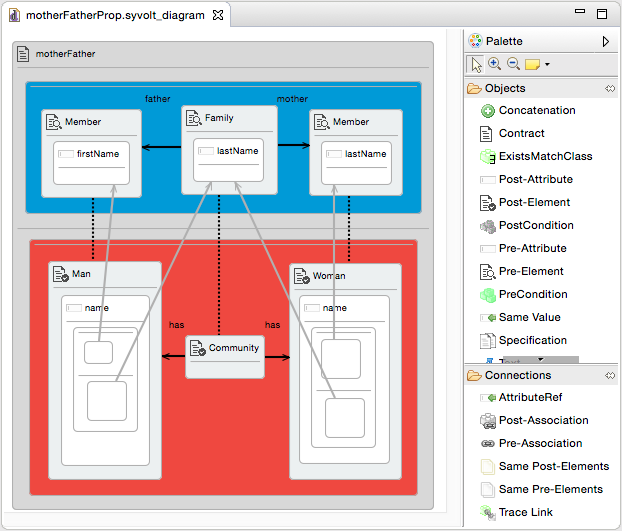
\includegraphics[width=0.5\textwidth]{figures/eclipse_frontend}
\caption{The transformation editor within Eclipse}
\label{fig:eclipse_frontend}
\end{figure}




 

\section{Architecture}
\label{sec:arch}
\begin{figure}
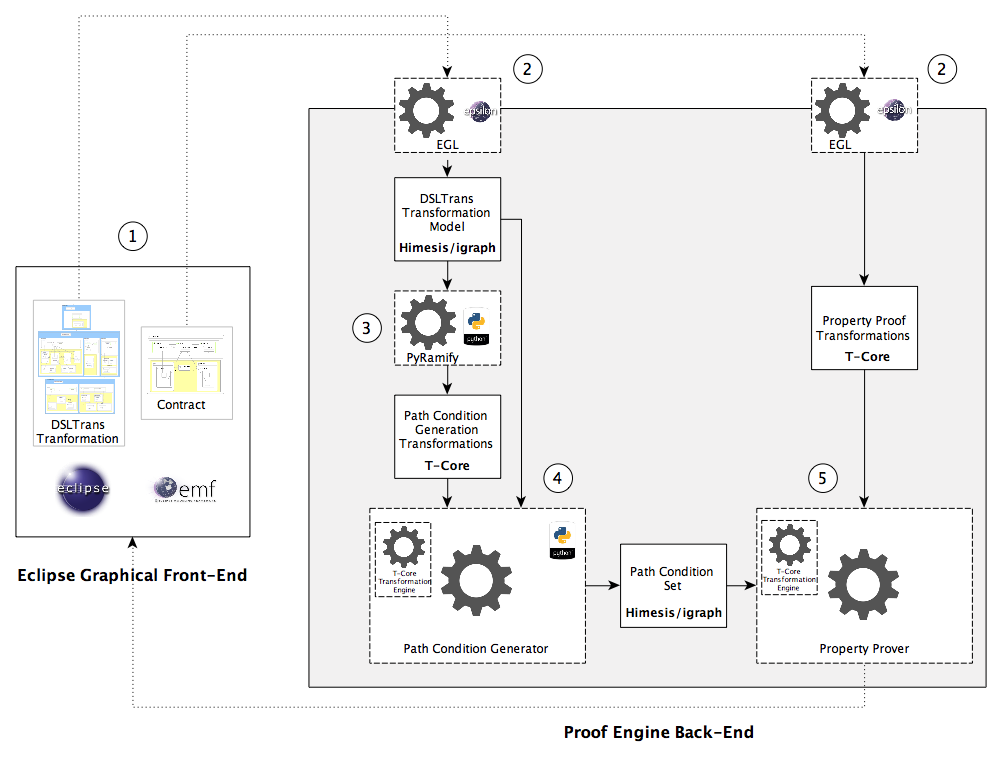
\includegraphics[width=0.45\textwidth]{figures/syvolt_arch}
\caption{The architecture of the SyVOLT tool}
\label{fig:arch}
\end{figure}

Figure~\ref{fig:arch} shows the architecture of the SyVOLT tool. We will now briefly visit each component in turn, mentioning the main technologies and languages employed.

Everything is a model or a transformation.



An Ant[CITE] script is then run from within the Eclipse environment. This script will orchestrate the following components.


\subsection{Generating Artifacts}
For our contract prover, there are a number of artifacts that need to be generated. For example, typed graphs (in the Himesis format[CITE]) are generated from each rule and contract, using the Eclipse Generation Language (EGL). As well, the top-level Python scripts used to prove contracts are also generated through this method.

This use of EGL allows for precise control over the artifacts that are produced, while taking a relatively short amount of time to create and debug.
Model-to-text generation.



\subsection{PyRamify}

PyRamify is a Python script that takes as input Himesis graphs representing the rules in the transformation. Then, through the RAMification procedure [CITE RAM], matchers for each rule are produced. These matchers will then match over the rules, which allows the contract prover to determine how rules might execute over an input model. Rewriters are also produced with traceability information, which will properly apply the right-hand side of a rule when it matches.

Currently, PyRamify is implemented as a Python script, as we were unable to implement automatic creation of higher-order artifacts in another modelling tool. We could not find technology to do higher-higher-order transformations. This is a limitation that we hope will be addressed. This led to a number of difficulties as PyRamify mixes together a number of different abstraction levels. 

\subsection{Use of T-Core}

T-Core, a blah blah blah, is used everywhere.


\subsection{Path Condition Generation}

Once the required artifacts have been produced, the prover moves onto the path condition generation step.  Each
path condition will represent a set of concrete executions
of the transformation, where each concrete execution is an
input/ouput pair.
Our proving algorithm begins by generating one empty
path condition, representing the case where no rules in the
transformation have executed. Then, each rule in each layer
is examined, and its graph is combined with the graph of
each path condition generated thus far. As each layer in the
transformation is considered, the set of path conditions will
grow to represent all allowed combinations of rules. As rules
may depend on each other because of backward links, such
dependencies are verified by the path condition generation
algorithm in order to exclude impossible rule combinations.
The final set of path conditions produced by the algorithm
will then abstract the infinite set of all concrete transformation
executions. This is further described in~\cite{Lucio2014}, along with a
formal discussion of the validity and completeness of this
work.

\subsection{Contract Proof}

Once the path conditions are generated, we can then begin the proof for each contract.

Pre- / post- condition contracts form an implication, which
needs to be checked for each path condition generated for
the transformation by the above algorithm. In broad terms,
a contract holds on a path condition if either the contract’s
pre-condition cannot be isomorphically found in the path
condition, or the contract’s pre-condition together with its post-
condition can be found in the path condition. The contract
does not hold on the path condition if its pre-condition can
be isomorphically found in the path condition but its post-
condition cannot. This produces a counter-example for the contract, which we then present to the user. Finally, a contract holds for a transformation if it holds for all of its generated path conditions. These results
are formally described in~\cite{Lucio2014}.

A contract holds in the transformation if, for all input models where the contract's pre-condition is found, the contract's post-condition is also found in the corresponding output model (with optional traceability constraints between the elements of the input and output models). Otherwise, the contract does not hold.







%
%\section{Mapping ATL into DSLTrans}
%\label{sec:mapping}
%\input{text/mapping}
%
%% \section{Transformation to DSLTrans}
%% \label{sec:transformation}
%% \input{text/hot}
%
%%\section{Properties and Property Prover}
%%\label{sec:prover}
%%\input{text/prover}
%
%\section{Results and Discussion}
%\label{sec:results}
%\input{text/results}
%
%
%\section{Related Work}
%\label{sec:related}
%\input{text/related}
%
\section{Summary}
\label{sec:conclusion}
%\input{text/conclusion}\vspace{-.5cm}

\section*{Acknowledgements}
The authors warmly thank Gehan Selim for her work on the
implementation of the contract prover. Bentley Oakes and Levi L\'ucio are
researchers working for the NECSIS project, funded by the Automotive Partnership
Canada. %The work of Javier Troya and Manuel Wimmer is funded by the European
%Commission under ICT Policy Support Programme, grant no. 317859.

\bibliographystyle{abbrv}
\bibliography{models2015}
\end{document}
